\documentclass[twoside]{book}

% Packages required by doxygen
\usepackage{fixltx2e}
\usepackage{calc}
\usepackage{doxygen}
\usepackage[export]{adjustbox} % also loads graphicx
\usepackage{graphicx}
\usepackage[utf8]{inputenc}
\usepackage{makeidx}
\usepackage{multicol}
\usepackage{multirow}
\PassOptionsToPackage{warn}{textcomp}
\usepackage{textcomp}
\usepackage[nointegrals]{wasysym}
\usepackage[table]{xcolor}

% NLS support packages
\usepackage[spanish]{babel}
% Font selection
\usepackage[T1]{fontenc}
\usepackage[scaled=.90]{helvet}
\usepackage{courier}
\usepackage{amssymb}
\usepackage{sectsty}
\renewcommand{\familydefault}{\sfdefault}
\allsectionsfont{%
  \fontseries{bc}\selectfont%
  \color{darkgray}%
}
\renewcommand{\DoxyLabelFont}{%
  \fontseries{bc}\selectfont%
  \color{darkgray}%
}
\newcommand{\+}{\discretionary{\mbox{\scriptsize$\hookleftarrow$}}{}{}}

% Page & text layout
\usepackage{geometry}
\geometry{%
  a4paper,%
  top=2.5cm,%
  bottom=2.5cm,%
  left=2.5cm,%
  right=2.5cm%
}
\tolerance=750
\hfuzz=15pt
\hbadness=750
\setlength{\emergencystretch}{15pt}
\setlength{\parindent}{0cm}
\setlength{\parskip}{3ex plus 2ex minus 2ex}
\makeatletter
\renewcommand{\paragraph}{%
  \@startsection{paragraph}{4}{0ex}{-1.0ex}{1.0ex}{%
    \normalfont\normalsize\bfseries\SS@parafont%
  }%
}
\renewcommand{\subparagraph}{%
  \@startsection{subparagraph}{5}{0ex}{-1.0ex}{1.0ex}{%
    \normalfont\normalsize\bfseries\SS@subparafont%
  }%
}
\makeatother

% Headers & footers
\usepackage{fancyhdr}
\pagestyle{fancyplain}
\fancyhead[LE]{\fancyplain{}{\bfseries\thepage}}
\fancyhead[CE]{\fancyplain{}{}}
\fancyhead[RE]{\fancyplain{}{\bfseries\leftmark}}
\fancyhead[LO]{\fancyplain{}{\bfseries\rightmark}}
\fancyhead[CO]{\fancyplain{}{}}
\fancyhead[RO]{\fancyplain{}{\bfseries\thepage}}
\fancyfoot[LE]{\fancyplain{}{}}
\fancyfoot[CE]{\fancyplain{}{}}
\fancyfoot[RE]{\fancyplain{}{\bfseries\scriptsize Generado por Doxygen }}
\fancyfoot[LO]{\fancyplain{}{\bfseries\scriptsize Generado por Doxygen }}
\fancyfoot[CO]{\fancyplain{}{}}
\fancyfoot[RO]{\fancyplain{}{}}
\renewcommand{\footrulewidth}{0.4pt}
\renewcommand{\chaptermark}[1]{%
  \markboth{#1}{}%
}
\renewcommand{\sectionmark}[1]{%
  \markright{\thesection\ #1}%
}

% Indices & bibliography
\usepackage{natbib}
\usepackage[titles]{tocloft}
\setcounter{tocdepth}{3}
\setcounter{secnumdepth}{5}
\makeindex

% Hyperlinks (required, but should be loaded last)
\usepackage{ifpdf}
\ifpdf
  \usepackage[pdftex,pagebackref=true]{hyperref}
\else
  \usepackage[ps2pdf,pagebackref=true]{hyperref}
\fi
\hypersetup{%
  colorlinks=true,%
  linkcolor=blue,%
  citecolor=blue,%
  unicode%
}

% Custom commands
\newcommand{\clearemptydoublepage}{%
  \newpage{\pagestyle{empty}\cleardoublepage}%
}

\usepackage{caption}
\captionsetup{labelsep=space,justification=centering,font={bf},singlelinecheck=off,skip=4pt,position=top}

%===== C O N T E N T S =====

\begin{document}

% Titlepage & ToC
\hypersetup{pageanchor=false,
             bookmarksnumbered=true,
             pdfencoding=unicode
            }
\pagenumbering{alph}
\begin{titlepage}
\vspace*{7cm}
\begin{center}%
{\Large Practica P\+R\+O2.\+Primavera 2020 \\[1ex]\large version 1 }\\
\vspace*{1cm}
{\large Generado por Doxygen 1.8.13}\\
\end{center}
\end{titlepage}
\clearemptydoublepage
\pagenumbering{roman}
\tableofcontents
\clearemptydoublepage
\pagenumbering{arabic}
\hypersetup{pageanchor=true}

%--- Begin generated contents ---
\chapter{Práctica P\+R\+O2}
\label{index}\hypertarget{index}{}\input{index}
\chapter{Índice de clases}
\section{Lista de clases}
Lista de las clases, estructuras, uniones e interfaces con una breve descripción\+:\begin{DoxyCompactList}
\item\contentsline{section}{\hyperlink{class_bin_tree}{Bin\+Tree$<$ T $>$} }{\pageref{class_bin_tree}}{}
\item\contentsline{section}{\hyperlink{class_cjt___clusters}{Cjt\+\_\+\+Clusters} \\*Representa una \hyperlink{class_cjt___clusters}{Cjt\+\_\+\+Clusters} }{\pageref{class_cjt___clusters}}{}
\item\contentsline{section}{\hyperlink{class_cjt___especies}{Cjt\+\_\+\+Especies} \\*Representa una \hyperlink{class_cjt___especies}{Cjt\+\_\+\+Especies} }{\pageref{class_cjt___especies}}{}
\item\contentsline{section}{\hyperlink{class_especie}{Especie} \\*Representa una especie }{\pageref{class_especie}}{}
\item\contentsline{section}{\hyperlink{class_taula__de__distancies}{Taula\+\_\+de\+\_\+distancies} \\*Representa una \hyperlink{class_taula__de__distancies}{Taula\+\_\+de\+\_\+distancies} }{\pageref{class_taula__de__distancies}}{}
\end{DoxyCompactList}

\chapter{Indice de archivos}
\section{Lista de archivos}
Lista de todos los archivos con descripciones breves\+:\begin{DoxyCompactList}
\item\contentsline{section}{\hyperlink{_bin_tree_8hh}{Bin\+Tree.\+hh} }{\pageref{_bin_tree_8hh}}{}
\item\contentsline{section}{\hyperlink{_cjt___clusters_8hh}{Cjt\+\_\+\+Clusters.\+hh} \\*Especificación de la clase \hyperlink{class_cjt___clusters}{Cjt\+\_\+\+Clusters} }{\pageref{_cjt___clusters_8hh}}{}
\item\contentsline{section}{\hyperlink{_cjt___especies_8hh}{Cjt\+\_\+\+Especies.\+hh} \\*Especificación de la clase \hyperlink{class_cjt___especies}{Cjt\+\_\+\+Especies} }{\pageref{_cjt___especies_8hh}}{}
\item\contentsline{section}{\hyperlink{_especie_8hh}{Especie.\+hh} \\*Especificación de la clase \hyperlink{class_especie}{Especie} }{\pageref{_especie_8hh}}{}
\item\contentsline{section}{\hyperlink{program_8cc}{program.\+cc} \\*Programa principal para el ejercicio {\itshape Practica P\+R\+O2.\+Primavera 2020} }{\pageref{program_8cc}}{}
\item\contentsline{section}{\hyperlink{_taula__de__distancies_8hh}{Taula\+\_\+de\+\_\+distancies.\+hh} \\*Especificación de la clase \hyperlink{class_taula__de__distancies}{Taula\+\_\+de\+\_\+distancies} }{\pageref{_taula__de__distancies_8hh}}{}
\end{DoxyCompactList}

\chapter{Documentación de las clases}
\hypertarget{class_bin_tree}{}\section{Referencia de la plantilla de la Clase Bin\+Tree$<$ T $>$}
\label{class_bin_tree}\index{Bin\+Tree$<$ T $>$@{Bin\+Tree$<$ T $>$}}
\subsection*{Métodos públicos}
\begin{DoxyCompactItemize}
\item 
\hyperlink{class_bin_tree_a47eef22d29cd023449d97c073c08e5b6}{Bin\+Tree} ()
\item 
\hyperlink{class_bin_tree_a1ab686e0bcf990093ff91fe71744c1a4}{Bin\+Tree} (const T \&x)
\item 
\hyperlink{class_bin_tree_adb7eeff76d08130c943b36af215eb521}{Bin\+Tree} (const T \&x, const \hyperlink{class_bin_tree}{Bin\+Tree} \&\hyperlink{class_bin_tree_a82108db4c1b08d1f111027788c196d4e}{left}, const \hyperlink{class_bin_tree}{Bin\+Tree} \&\hyperlink{class_bin_tree_aff8e96651b27284c329667b5ad3e4d0b}{right})
\item 
bool \hyperlink{class_bin_tree_a74cda259ba5c25b8ee38ed4dc33e4fad}{empty} () const
\item 
\hyperlink{class_bin_tree}{Bin\+Tree} \hyperlink{class_bin_tree_a82108db4c1b08d1f111027788c196d4e}{left} () const
\item 
\hyperlink{class_bin_tree}{Bin\+Tree} \hyperlink{class_bin_tree_aff8e96651b27284c329667b5ad3e4d0b}{right} () const
\item 
const T \& \hyperlink{class_bin_tree_a734e785b089c87b49187ee7c58edf5f3}{value} () const
\end{DoxyCompactItemize}


\subsection{Descripción detallada}
\subsubsection*{template$<$typename T$>$\newline
class Bin\+Tree$<$ T $>$}



Definición en la línea 12 del archivo Bin\+Tree.\+hh.



\subsection{Documentación del constructor y destructor}
\mbox{\Hypertarget{class_bin_tree_a47eef22d29cd023449d97c073c08e5b6}\label{class_bin_tree_a47eef22d29cd023449d97c073c08e5b6}} 
\index{Bin\+Tree@{Bin\+Tree}!Bin\+Tree@{Bin\+Tree}}
\index{Bin\+Tree@{Bin\+Tree}!Bin\+Tree@{Bin\+Tree}}
\subsubsection{\texorpdfstring{Bin\+Tree()}{BinTree()}\hspace{0.1cm}{\footnotesize\ttfamily [1/3]}}
{\footnotesize\ttfamily template$<$typename T$>$ \\
\hyperlink{class_bin_tree}{Bin\+Tree}$<$ T $>$\+::\hyperlink{class_bin_tree}{Bin\+Tree} (\begin{DoxyParamCaption}{ }\end{DoxyParamCaption})}



Definición en la línea 41 del archivo Bin\+Tree.\+hh.


\begin{DoxyCode}
42     :   p(\textcolor{keyword}{nullptr})
43     \{   \}
\end{DoxyCode}
\mbox{\Hypertarget{class_bin_tree_a1ab686e0bcf990093ff91fe71744c1a4}\label{class_bin_tree_a1ab686e0bcf990093ff91fe71744c1a4}} 
\index{Bin\+Tree@{Bin\+Tree}!Bin\+Tree@{Bin\+Tree}}
\index{Bin\+Tree@{Bin\+Tree}!Bin\+Tree@{Bin\+Tree}}
\subsubsection{\texorpdfstring{Bin\+Tree()}{BinTree()}\hspace{0.1cm}{\footnotesize\ttfamily [2/3]}}
{\footnotesize\ttfamily template$<$typename T$>$ \\
\hyperlink{class_bin_tree}{Bin\+Tree}$<$ T $>$\+::\hyperlink{class_bin_tree}{Bin\+Tree} (\begin{DoxyParamCaption}\item[{const T \&}]{x }\end{DoxyParamCaption})}



Definición en la línea 46 del archivo Bin\+Tree.\+hh.


\begin{DoxyCode}
46                          \{
47         p = make\_shared<Node>(x, \textcolor{keyword}{nullptr}, \textcolor{keyword}{nullptr});
48     \}
\end{DoxyCode}
\mbox{\Hypertarget{class_bin_tree_adb7eeff76d08130c943b36af215eb521}\label{class_bin_tree_adb7eeff76d08130c943b36af215eb521}} 
\index{Bin\+Tree@{Bin\+Tree}!Bin\+Tree@{Bin\+Tree}}
\index{Bin\+Tree@{Bin\+Tree}!Bin\+Tree@{Bin\+Tree}}
\subsubsection{\texorpdfstring{Bin\+Tree()}{BinTree()}\hspace{0.1cm}{\footnotesize\ttfamily [3/3]}}
{\footnotesize\ttfamily template$<$typename T$>$ \\
\hyperlink{class_bin_tree}{Bin\+Tree}$<$ T $>$\+::\hyperlink{class_bin_tree}{Bin\+Tree} (\begin{DoxyParamCaption}\item[{const T \&}]{x,  }\item[{const \hyperlink{class_bin_tree}{Bin\+Tree}$<$ T $>$ \&}]{left,  }\item[{const \hyperlink{class_bin_tree}{Bin\+Tree}$<$ T $>$ \&}]{right }\end{DoxyParamCaption})}



Definición en la línea 51 del archivo Bin\+Tree.\+hh.


\begin{DoxyCode}
51                                                                     \{
52         p = make\_shared<Node>(x, left.p, right.p);
53     \}
\end{DoxyCode}


\subsection{Documentación de las funciones miembro}
\mbox{\Hypertarget{class_bin_tree_a74cda259ba5c25b8ee38ed4dc33e4fad}\label{class_bin_tree_a74cda259ba5c25b8ee38ed4dc33e4fad}} 
\index{Bin\+Tree@{Bin\+Tree}!empty@{empty}}
\index{empty@{empty}!Bin\+Tree@{Bin\+Tree}}
\subsubsection{\texorpdfstring{empty()}{empty()}}
{\footnotesize\ttfamily template$<$typename T$>$ \\
bool \hyperlink{class_bin_tree}{Bin\+Tree}$<$ T $>$\+::empty (\begin{DoxyParamCaption}{ }\end{DoxyParamCaption}) const}



Definición en la línea 56 del archivo Bin\+Tree.\+hh.


\begin{DoxyCode}
56                         \{
57         \textcolor{keywordflow}{return} not p;
58     \}
\end{DoxyCode}
\mbox{\Hypertarget{class_bin_tree_a82108db4c1b08d1f111027788c196d4e}\label{class_bin_tree_a82108db4c1b08d1f111027788c196d4e}} 
\index{Bin\+Tree@{Bin\+Tree}!left@{left}}
\index{left@{left}!Bin\+Tree@{Bin\+Tree}}
\subsubsection{\texorpdfstring{left()}{left()}}
{\footnotesize\ttfamily template$<$typename T$>$ \\
\hyperlink{class_bin_tree}{Bin\+Tree} \hyperlink{class_bin_tree}{Bin\+Tree}$<$ T $>$\+::left (\begin{DoxyParamCaption}{ }\end{DoxyParamCaption}) const}



Definición en la línea 61 del archivo Bin\+Tree.\+hh.


\begin{DoxyCode}
61                           \{
62         assert(not \hyperlink{class_bin_tree_a74cda259ba5c25b8ee38ed4dc33e4fad}{empty}());
63         \textcolor{keywordflow}{return} \hyperlink{class_bin_tree_a47eef22d29cd023449d97c073c08e5b6}{BinTree}(p->left);
64     \}
\end{DoxyCode}
\mbox{\Hypertarget{class_bin_tree_aff8e96651b27284c329667b5ad3e4d0b}\label{class_bin_tree_aff8e96651b27284c329667b5ad3e4d0b}} 
\index{Bin\+Tree@{Bin\+Tree}!right@{right}}
\index{right@{right}!Bin\+Tree@{Bin\+Tree}}
\subsubsection{\texorpdfstring{right()}{right()}}
{\footnotesize\ttfamily template$<$typename T$>$ \\
\hyperlink{class_bin_tree}{Bin\+Tree} \hyperlink{class_bin_tree}{Bin\+Tree}$<$ T $>$\+::right (\begin{DoxyParamCaption}{ }\end{DoxyParamCaption}) const}



Definición en la línea 67 del archivo Bin\+Tree.\+hh.


\begin{DoxyCode}
67                            \{
68         assert(not \hyperlink{class_bin_tree_a74cda259ba5c25b8ee38ed4dc33e4fad}{empty}());
69         \textcolor{keywordflow}{return} \hyperlink{class_bin_tree_a47eef22d29cd023449d97c073c08e5b6}{BinTree}(p->right);
70     \}
\end{DoxyCode}
\mbox{\Hypertarget{class_bin_tree_a734e785b089c87b49187ee7c58edf5f3}\label{class_bin_tree_a734e785b089c87b49187ee7c58edf5f3}} 
\index{Bin\+Tree@{Bin\+Tree}!value@{value}}
\index{value@{value}!Bin\+Tree@{Bin\+Tree}}
\subsubsection{\texorpdfstring{value()}{value()}}
{\footnotesize\ttfamily template$<$typename T$>$ \\
const T\& \hyperlink{class_bin_tree}{Bin\+Tree}$<$ T $>$\+::value (\begin{DoxyParamCaption}{ }\end{DoxyParamCaption}) const}



Definición en la línea 73 del archivo Bin\+Tree.\+hh.


\begin{DoxyCode}
73                             \{
74         assert(not \hyperlink{class_bin_tree_a74cda259ba5c25b8ee38ed4dc33e4fad}{empty}());
75         \textcolor{keywordflow}{return} p->x;
76     \}
\end{DoxyCode}


La documentación para esta clase fue generada a partir del siguiente fichero\+:\begin{DoxyCompactItemize}
\item 
\hyperlink{_bin_tree_8hh}{Bin\+Tree.\+hh}\end{DoxyCompactItemize}

\hypertarget{class_cjt___clusters}{}\section{Referencia de la Clase Cjt\+\_\+\+Clusters}
\label{class_cjt___clusters}\index{Cjt\+\_\+\+Clusters@{Cjt\+\_\+\+Clusters}}


Representa una \hyperlink{class_cjt___clusters}{Cjt\+\_\+\+Clusters}.  


\subsection*{Métodos públicos}
\begin{DoxyCompactItemize}
\item 
\hyperlink{class_cjt___clusters_a2e55759944a78043744103e19dd87c1c}{Cjt\+\_\+\+Clusters} ()
\begin{DoxyCompactList}\small\item\em Creadora por defecto. \end{DoxyCompactList}\item 
void \hyperlink{class_cjt___clusters_a7dec4a423a1dbcf6d0351e00dd653eee}{inicializa\+\_\+clusters} (\hyperlink{class_cjt___especies}{Cjt\+\_\+\+Especies} \&Mostra, \hyperlink{class_taula__de__distancies}{Taula\+\_\+de\+\_\+distancies} \&Taula)
\begin{DoxyCompactList}\small\item\em Modificadora de inicializa el clúster. \end{DoxyCompactList}\item 
void \hyperlink{class_cjt___clusters_a1656b81e5200625b44c8f138c09af068}{ejecutar\+\_\+paso\+\_\+wpgma} ()
\begin{DoxyCompactList}\small\item\em Modificadora de ejecutar paso wpgma. \end{DoxyCompactList}\item 
void \hyperlink{class_cjt___clusters_a284f66b3e8c47eded1e24af805b81505}{imprime\+\_\+cluster} (\hyperlink{class_bin_tree}{Bin\+Tree}$<$ pair$<$ string, double $>$$>$ arbre)
\begin{DoxyCompactList}\small\item\em Operación de escritura. \end{DoxyCompactList}\item 
void \hyperlink{class_cjt___clusters_a19510eceda5d5bf39d7091a28bf5f00c}{imprime\+\_\+cluster\+\_\+aux} (\hyperlink{class_bin_tree}{Bin\+Tree}$<$ pair$<$ string, double $>$$>$ \&arbre)
\begin{DoxyCompactList}\small\item\em Operación de escritura. \end{DoxyCompactList}\item 
void \hyperlink{class_cjt___clusters_a95262506a2fdc5455ce104fb84649ee9}{imprime\+\_\+arbol\+\_\+filogenetico} ()
\begin{DoxyCompactList}\small\item\em Operación de escritura. \end{DoxyCompactList}\item 
void \hyperlink{class_cjt___clusters_a6a261f0f5ca471e257d6b17e91b4887a}{taula\+\_\+clusters\+\_\+imprime} ()
\begin{DoxyCompactList}\small\item\em Operación de escritura. \end{DoxyCompactList}\item 
bool \hyperlink{class_cjt___clusters_a4fcda36a68e8fe48d787dfd14e9b222b}{existe\+\_\+cluster} (string id)
\begin{DoxyCompactList}\small\item\em Consultora existencia de cluster. \end{DoxyCompactList}\item 
int \hyperlink{class_cjt___clusters_ad00d2fe80f0b0dc1e593a91f8be6b761}{numero\+\_\+clusters} ()
\begin{DoxyCompactList}\small\item\em Consultora del tamaño del conjunto de clusters. \end{DoxyCompactList}\item 
\hyperlink{class_bin_tree}{Bin\+Tree}$<$ pair$<$ string, double $>$ $>$ \hyperlink{class_cjt___clusters_aca3506a7084d53e251ff052b0bbaf5bb}{retorna\+\_\+subarb} (string id)
\begin{DoxyCompactList}\small\item\em Consultora del clusters. \end{DoxyCompactList}\end{DoxyCompactItemize}


\subsection{Descripción detallada}
Representa una \hyperlink{class_cjt___clusters}{Cjt\+\_\+\+Clusters}. 

Contiene un \hyperlink{class_bin_tree}{Bin\+Tree} formado por el \hyperlink{class_cjt___especies}{Cjt\+\_\+\+Especies} 

Definición en la línea 22 del archivo Cjt\+\_\+\+Clusters.\+hh.



\subsection{Documentación del constructor y destructor}
\mbox{\Hypertarget{class_cjt___clusters_a2e55759944a78043744103e19dd87c1c}\label{class_cjt___clusters_a2e55759944a78043744103e19dd87c1c}} 
\index{Cjt\+\_\+\+Clusters@{Cjt\+\_\+\+Clusters}!Cjt\+\_\+\+Clusters@{Cjt\+\_\+\+Clusters}}
\index{Cjt\+\_\+\+Clusters@{Cjt\+\_\+\+Clusters}!Cjt\+\_\+\+Clusters@{Cjt\+\_\+\+Clusters}}
\subsubsection{\texorpdfstring{Cjt\+\_\+\+Clusters()}{Cjt\_Clusters()}}
{\footnotesize\ttfamily Cjt\+\_\+\+Clusters\+::\+Cjt\+\_\+\+Clusters (\begin{DoxyParamCaption}{ }\end{DoxyParamCaption})}



Creadora por defecto. 

\begin{DoxyPrecond}{Precondición}
{\itshape cierto} 
\end{DoxyPrecond}
\begin{DoxyPostcond}{Postcondición}
El resultado es un conjunto de clusters vacío 
\end{DoxyPostcond}


\subsection{Documentación de las funciones miembro}
\mbox{\Hypertarget{class_cjt___clusters_a7dec4a423a1dbcf6d0351e00dd653eee}\label{class_cjt___clusters_a7dec4a423a1dbcf6d0351e00dd653eee}} 
\index{Cjt\+\_\+\+Clusters@{Cjt\+\_\+\+Clusters}!inicializa\+\_\+clusters@{inicializa\+\_\+clusters}}
\index{inicializa\+\_\+clusters@{inicializa\+\_\+clusters}!Cjt\+\_\+\+Clusters@{Cjt\+\_\+\+Clusters}}
\subsubsection{\texorpdfstring{inicializa\+\_\+clusters()}{inicializa\_clusters()}}
{\footnotesize\ttfamily void Cjt\+\_\+\+Clusters\+::inicializa\+\_\+clusters (\begin{DoxyParamCaption}\item[{\hyperlink{class_cjt___especies}{Cjt\+\_\+\+Especies} \&}]{Mostra,  }\item[{\hyperlink{class_taula__de__distancies}{Taula\+\_\+de\+\_\+distancies} \&}]{Taula }\end{DoxyParamCaption})}



Modificadora de inicializa el clúster. 

\begin{DoxyPrecond}{Precondición}
{\itshape cierto} 
\end{DoxyPrecond}
\begin{DoxyPostcond}{Postcondición}
Inicializa el conjunto de clúsers con el conjunto de especies end el estado en el que esté en ese momento e imprime los clústers resultantes, así como la tabla de distancias 
\end{DoxyPostcond}
\mbox{\Hypertarget{class_cjt___clusters_a1656b81e5200625b44c8f138c09af068}\label{class_cjt___clusters_a1656b81e5200625b44c8f138c09af068}} 
\index{Cjt\+\_\+\+Clusters@{Cjt\+\_\+\+Clusters}!ejecutar\+\_\+paso\+\_\+wpgma@{ejecutar\+\_\+paso\+\_\+wpgma}}
\index{ejecutar\+\_\+paso\+\_\+wpgma@{ejecutar\+\_\+paso\+\_\+wpgma}!Cjt\+\_\+\+Clusters@{Cjt\+\_\+\+Clusters}}
\subsubsection{\texorpdfstring{ejecutar\+\_\+paso\+\_\+wpgma()}{ejecutar\_paso\_wpgma()}}
{\footnotesize\ttfamily void Cjt\+\_\+\+Clusters\+::ejecutar\+\_\+paso\+\_\+wpgma (\begin{DoxyParamCaption}{ }\end{DoxyParamCaption})}



Modificadora de ejecutar paso wpgma. 

\begin{DoxyPrecond}{Precondición}
{\itshape cierto} 
\end{DoxyPrecond}
\begin{DoxyPostcond}{Postcondición}
El resultado es la creación de un nuevo cluster con las distancias calculadas y la eliminación de los clusters con distancia mas pequeña 
\end{DoxyPostcond}
\mbox{\Hypertarget{class_cjt___clusters_a284f66b3e8c47eded1e24af805b81505}\label{class_cjt___clusters_a284f66b3e8c47eded1e24af805b81505}} 
\index{Cjt\+\_\+\+Clusters@{Cjt\+\_\+\+Clusters}!imprime\+\_\+cluster@{imprime\+\_\+cluster}}
\index{imprime\+\_\+cluster@{imprime\+\_\+cluster}!Cjt\+\_\+\+Clusters@{Cjt\+\_\+\+Clusters}}
\subsubsection{\texorpdfstring{imprime\+\_\+cluster()}{imprime\_cluster()}}
{\footnotesize\ttfamily void Cjt\+\_\+\+Clusters\+::imprime\+\_\+cluster (\begin{DoxyParamCaption}\item[{\hyperlink{class_bin_tree}{Bin\+Tree}$<$ pair$<$ string, double $>$$>$}]{arbre }\end{DoxyParamCaption})}



Operación de escritura. 

\begin{DoxyPrecond}{Precondición}
{\itshape cierto} 
\end{DoxyPrecond}
\begin{DoxyPostcond}{Postcondición}
Escribe el contenido del parámetro implícito por el canal estándar de salida 
\end{DoxyPostcond}
\mbox{\Hypertarget{class_cjt___clusters_a19510eceda5d5bf39d7091a28bf5f00c}\label{class_cjt___clusters_a19510eceda5d5bf39d7091a28bf5f00c}} 
\index{Cjt\+\_\+\+Clusters@{Cjt\+\_\+\+Clusters}!imprime\+\_\+cluster\+\_\+aux@{imprime\+\_\+cluster\+\_\+aux}}
\index{imprime\+\_\+cluster\+\_\+aux@{imprime\+\_\+cluster\+\_\+aux}!Cjt\+\_\+\+Clusters@{Cjt\+\_\+\+Clusters}}
\subsubsection{\texorpdfstring{imprime\+\_\+cluster\+\_\+aux()}{imprime\_cluster\_aux()}}
{\footnotesize\ttfamily void Cjt\+\_\+\+Clusters\+::imprime\+\_\+cluster\+\_\+aux (\begin{DoxyParamCaption}\item[{\hyperlink{class_bin_tree}{Bin\+Tree}$<$ pair$<$ string, double $>$$>$ \&}]{arbre }\end{DoxyParamCaption})}



Operación de escritura. 

\begin{DoxyPrecond}{Precondición}
{\itshape cierto} 
\end{DoxyPrecond}
\begin{DoxyPostcond}{Postcondición}
llama a la función imprime\+\_\+cluster y hace un salto de linea 
\end{DoxyPostcond}
\mbox{\Hypertarget{class_cjt___clusters_a95262506a2fdc5455ce104fb84649ee9}\label{class_cjt___clusters_a95262506a2fdc5455ce104fb84649ee9}} 
\index{Cjt\+\_\+\+Clusters@{Cjt\+\_\+\+Clusters}!imprime\+\_\+arbol\+\_\+filogenetico@{imprime\+\_\+arbol\+\_\+filogenetico}}
\index{imprime\+\_\+arbol\+\_\+filogenetico@{imprime\+\_\+arbol\+\_\+filogenetico}!Cjt\+\_\+\+Clusters@{Cjt\+\_\+\+Clusters}}
\subsubsection{\texorpdfstring{imprime\+\_\+arbol\+\_\+filogenetico()}{imprime\_arbol\_filogenetico()}}
{\footnotesize\ttfamily void Cjt\+\_\+\+Clusters\+::imprime\+\_\+arbol\+\_\+filogenetico (\begin{DoxyParamCaption}{ }\end{DoxyParamCaption})}



Operación de escritura. 

\begin{DoxyPrecond}{Precondición}
{\itshape cierto} 
\end{DoxyPrecond}
\begin{DoxyPostcond}{Postcondición}
Escribe el contenido del parámetro implícito por el canal estándar de salida 
\end{DoxyPostcond}
\mbox{\Hypertarget{class_cjt___clusters_a6a261f0f5ca471e257d6b17e91b4887a}\label{class_cjt___clusters_a6a261f0f5ca471e257d6b17e91b4887a}} 
\index{Cjt\+\_\+\+Clusters@{Cjt\+\_\+\+Clusters}!taula\+\_\+clusters\+\_\+imprime@{taula\+\_\+clusters\+\_\+imprime}}
\index{taula\+\_\+clusters\+\_\+imprime@{taula\+\_\+clusters\+\_\+imprime}!Cjt\+\_\+\+Clusters@{Cjt\+\_\+\+Clusters}}
\subsubsection{\texorpdfstring{taula\+\_\+clusters\+\_\+imprime()}{taula\_clusters\_imprime()}}
{\footnotesize\ttfamily void Cjt\+\_\+\+Clusters\+::taula\+\_\+clusters\+\_\+imprime (\begin{DoxyParamCaption}{ }\end{DoxyParamCaption})}



Operación de escritura. 

\begin{DoxyPrecond}{Precondición}
{\itshape cierto} 
\end{DoxyPrecond}
\begin{DoxyPostcond}{Postcondición}
Escribe el contenido del parámetro implícito por el canal estándar de salida 
\end{DoxyPostcond}
\mbox{\Hypertarget{class_cjt___clusters_a4fcda36a68e8fe48d787dfd14e9b222b}\label{class_cjt___clusters_a4fcda36a68e8fe48d787dfd14e9b222b}} 
\index{Cjt\+\_\+\+Clusters@{Cjt\+\_\+\+Clusters}!existe\+\_\+cluster@{existe\+\_\+cluster}}
\index{existe\+\_\+cluster@{existe\+\_\+cluster}!Cjt\+\_\+\+Clusters@{Cjt\+\_\+\+Clusters}}
\subsubsection{\texorpdfstring{existe\+\_\+cluster()}{existe\_cluster()}}
{\footnotesize\ttfamily bool Cjt\+\_\+\+Clusters\+::existe\+\_\+cluster (\begin{DoxyParamCaption}\item[{string}]{id }\end{DoxyParamCaption})}



Consultora existencia de cluster. 

\begin{DoxyPrecond}{Precondición}
{\itshape cierto} 
\end{DoxyPrecond}
\begin{DoxyPostcond}{Postcondición}
retorna true si existe y false si no 
\end{DoxyPostcond}
\mbox{\Hypertarget{class_cjt___clusters_ad00d2fe80f0b0dc1e593a91f8be6b761}\label{class_cjt___clusters_ad00d2fe80f0b0dc1e593a91f8be6b761}} 
\index{Cjt\+\_\+\+Clusters@{Cjt\+\_\+\+Clusters}!numero\+\_\+clusters@{numero\+\_\+clusters}}
\index{numero\+\_\+clusters@{numero\+\_\+clusters}!Cjt\+\_\+\+Clusters@{Cjt\+\_\+\+Clusters}}
\subsubsection{\texorpdfstring{numero\+\_\+clusters()}{numero\_clusters()}}
{\footnotesize\ttfamily int Cjt\+\_\+\+Clusters\+::numero\+\_\+clusters (\begin{DoxyParamCaption}{ }\end{DoxyParamCaption})}



Consultora del tamaño del conjunto de clusters. 

\begin{DoxyPrecond}{Precondición}
{\itshape cierto} 
\end{DoxyPrecond}
\begin{DoxyPostcond}{Postcondición}
retorna un int con el tamaño del conjunto de clusters 
\end{DoxyPostcond}
\mbox{\Hypertarget{class_cjt___clusters_aca3506a7084d53e251ff052b0bbaf5bb}\label{class_cjt___clusters_aca3506a7084d53e251ff052b0bbaf5bb}} 
\index{Cjt\+\_\+\+Clusters@{Cjt\+\_\+\+Clusters}!retorna\+\_\+subarb@{retorna\+\_\+subarb}}
\index{retorna\+\_\+subarb@{retorna\+\_\+subarb}!Cjt\+\_\+\+Clusters@{Cjt\+\_\+\+Clusters}}
\subsubsection{\texorpdfstring{retorna\+\_\+subarb()}{retorna\_subarb()}}
{\footnotesize\ttfamily \hyperlink{class_bin_tree}{Bin\+Tree}$<$pair$<$string,double$>$ $>$ Cjt\+\_\+\+Clusters\+::retorna\+\_\+subarb (\begin{DoxyParamCaption}\item[{string}]{id }\end{DoxyParamCaption})}



Consultora del clusters. 

\begin{DoxyPrecond}{Precondición}
{\itshape cierto} 
\end{DoxyPrecond}
\begin{DoxyPostcond}{Postcondición}
retorna el \hyperlink{class_bin_tree}{Bin\+Tree} donde se encuentra el string que entra 
\end{DoxyPostcond}


La documentación para esta clase fue generada a partir del siguiente fichero\+:\begin{DoxyCompactItemize}
\item 
\hyperlink{_cjt___clusters_8hh}{Cjt\+\_\+\+Clusters.\+hh}\end{DoxyCompactItemize}

\hypertarget{class_cjt___especies}{}\section{Referencia de la Clase Cjt\+\_\+\+Especies}
\label{class_cjt___especies}\index{Cjt\+\_\+\+Especies@{Cjt\+\_\+\+Especies}}


Representa una \hyperlink{class_cjt___especies}{Cjt\+\_\+\+Especies}.  


\subsection*{Métodos públicos}
\begin{DoxyCompactItemize}
\item 
\hyperlink{class_cjt___especies_ae423b9d5a456158136c17d9210c90c2e}{Cjt\+\_\+\+Especies} ()
\begin{DoxyCompactList}\small\item\em Creadora por defecto. \end{DoxyCompactList}\item 
void \hyperlink{class_cjt___especies_a8c90cec35ff5469f0b8e193308569e4b}{crea\+\_\+especie} (string id, string gen, int k)
\begin{DoxyCompactList}\small\item\em Modificadora de creación de especie. \end{DoxyCompactList}\item 
void \hyperlink{class_cjt___especies_aef76f607ead23a635d7a8b2c9a844327}{elimina\+\_\+especie} (string id)
\begin{DoxyCompactList}\small\item\em Modificadora de eliminación de especie. \end{DoxyCompactList}\item 
bool \hyperlink{class_cjt___especies_a39a4191697228fea8780516f4cd5da85}{existe\+\_\+especie} (string id)
\begin{DoxyCompactList}\small\item\em Consultora del especie. \end{DoxyCompactList}\item 
string \hyperlink{class_cjt___especies_af5821877f200218836053864ba8e9462}{obtener\+\_\+gen} (string id)
\begin{DoxyCompactList}\small\item\em Consultora del gen. \end{DoxyCompactList}\item 
vector$<$ string $>$ \hyperlink{class_cjt___especies_a8b79c4a271c4d5e4f6c3aa1b8b69b9ec}{obtener\+\_\+sub\+\_\+gen} (string id)
\begin{DoxyCompactList}\small\item\em Consultora del sub\+\_\+gen. \end{DoxyCompactList}\item 
void \hyperlink{class_cjt___especies_a341dfedcac85d19e084d68f7611af8f9}{eliminar\+\_\+totes} ()
\begin{DoxyCompactList}\small\item\em Operación de lectura. \end{DoxyCompactList}\item 
void \hyperlink{class_cjt___especies_a61b0168970e926d3a27faf3f31ad2869}{imprime\+\_\+cjt\+\_\+especies} ()
\begin{DoxyCompactList}\small\item\em Operación de escriptura. \end{DoxyCompactList}\item 
vector$<$ string $>$ \hyperlink{class_cjt___especies_aa06bb16bd1733ed2985bb312d3c8d42b}{retorna\+\_\+especies} ()
\begin{DoxyCompactList}\small\item\em Consultora del id del cjt\+\_\+especies. \end{DoxyCompactList}\end{DoxyCompactItemize}


\subsection{Descripción detallada}
Representa una \hyperlink{class_cjt___especies}{Cjt\+\_\+\+Especies}. 

Contiene un map formado por dos strings 

Definición en la línea 19 del archivo Cjt\+\_\+\+Especies.\+hh.



\subsection{Documentación del constructor y destructor}
\mbox{\Hypertarget{class_cjt___especies_ae423b9d5a456158136c17d9210c90c2e}\label{class_cjt___especies_ae423b9d5a456158136c17d9210c90c2e}} 
\index{Cjt\+\_\+\+Especies@{Cjt\+\_\+\+Especies}!Cjt\+\_\+\+Especies@{Cjt\+\_\+\+Especies}}
\index{Cjt\+\_\+\+Especies@{Cjt\+\_\+\+Especies}!Cjt\+\_\+\+Especies@{Cjt\+\_\+\+Especies}}
\subsubsection{\texorpdfstring{Cjt\+\_\+\+Especies()}{Cjt\_Especies()}}
{\footnotesize\ttfamily Cjt\+\_\+\+Especies\+::\+Cjt\+\_\+\+Especies (\begin{DoxyParamCaption}{ }\end{DoxyParamCaption})}



Creadora por defecto. 

\begin{DoxyPrecond}{Precondición}
{\itshape cierto} 
\end{DoxyPrecond}
\begin{DoxyPostcond}{Postcondición}
El resultado es un conjunto de especies vacío 
\end{DoxyPostcond}


\subsection{Documentación de las funciones miembro}
\mbox{\Hypertarget{class_cjt___especies_a8c90cec35ff5469f0b8e193308569e4b}\label{class_cjt___especies_a8c90cec35ff5469f0b8e193308569e4b}} 
\index{Cjt\+\_\+\+Especies@{Cjt\+\_\+\+Especies}!crea\+\_\+especie@{crea\+\_\+especie}}
\index{crea\+\_\+especie@{crea\+\_\+especie}!Cjt\+\_\+\+Especies@{Cjt\+\_\+\+Especies}}
\subsubsection{\texorpdfstring{crea\+\_\+especie()}{crea\_especie()}}
{\footnotesize\ttfamily void Cjt\+\_\+\+Especies\+::crea\+\_\+especie (\begin{DoxyParamCaption}\item[{string}]{id,  }\item[{string}]{gen,  }\item[{int}]{k }\end{DoxyParamCaption})}



Modificadora de creación de especie. 

\begin{DoxyPrecond}{Precondición}
{\itshape cierto} 
\end{DoxyPrecond}
\begin{DoxyPostcond}{Postcondición}
El resultado es una nueva especie en el map 
\end{DoxyPostcond}
\mbox{\Hypertarget{class_cjt___especies_aef76f607ead23a635d7a8b2c9a844327}\label{class_cjt___especies_aef76f607ead23a635d7a8b2c9a844327}} 
\index{Cjt\+\_\+\+Especies@{Cjt\+\_\+\+Especies}!elimina\+\_\+especie@{elimina\+\_\+especie}}
\index{elimina\+\_\+especie@{elimina\+\_\+especie}!Cjt\+\_\+\+Especies@{Cjt\+\_\+\+Especies}}
\subsubsection{\texorpdfstring{elimina\+\_\+especie()}{elimina\_especie()}}
{\footnotesize\ttfamily void Cjt\+\_\+\+Especies\+::elimina\+\_\+especie (\begin{DoxyParamCaption}\item[{string}]{id }\end{DoxyParamCaption})}



Modificadora de eliminación de especie. 

\begin{DoxyPrecond}{Precondición}
{\itshape cierto} 
\end{DoxyPrecond}
\begin{DoxyPostcond}{Postcondición}
El resultado es la eliminación de una especie del conjunto de especies 
\end{DoxyPostcond}
\mbox{\Hypertarget{class_cjt___especies_a39a4191697228fea8780516f4cd5da85}\label{class_cjt___especies_a39a4191697228fea8780516f4cd5da85}} 
\index{Cjt\+\_\+\+Especies@{Cjt\+\_\+\+Especies}!existe\+\_\+especie@{existe\+\_\+especie}}
\index{existe\+\_\+especie@{existe\+\_\+especie}!Cjt\+\_\+\+Especies@{Cjt\+\_\+\+Especies}}
\subsubsection{\texorpdfstring{existe\+\_\+especie()}{existe\_especie()}}
{\footnotesize\ttfamily bool Cjt\+\_\+\+Especies\+::existe\+\_\+especie (\begin{DoxyParamCaption}\item[{string}]{id }\end{DoxyParamCaption})}



Consultora del especie. 

\begin{DoxyPrecond}{Precondición}
{\itshape cierto} 
\end{DoxyPrecond}
\begin{DoxyPostcond}{Postcondición}
El resultado es true si existe i false i no 
\end{DoxyPostcond}
\mbox{\Hypertarget{class_cjt___especies_af5821877f200218836053864ba8e9462}\label{class_cjt___especies_af5821877f200218836053864ba8e9462}} 
\index{Cjt\+\_\+\+Especies@{Cjt\+\_\+\+Especies}!obtener\+\_\+gen@{obtener\+\_\+gen}}
\index{obtener\+\_\+gen@{obtener\+\_\+gen}!Cjt\+\_\+\+Especies@{Cjt\+\_\+\+Especies}}
\subsubsection{\texorpdfstring{obtener\+\_\+gen()}{obtener\_gen()}}
{\footnotesize\ttfamily string Cjt\+\_\+\+Especies\+::obtener\+\_\+gen (\begin{DoxyParamCaption}\item[{string}]{id }\end{DoxyParamCaption})}



Consultora del gen. 

\begin{DoxyPrecond}{Precondición}
{\itshape cierto} 
\end{DoxyPrecond}
\begin{DoxyPostcond}{Postcondición}
El resultado es el gen correspondiente al identificador dado 
\end{DoxyPostcond}
\mbox{\Hypertarget{class_cjt___especies_a8b79c4a271c4d5e4f6c3aa1b8b69b9ec}\label{class_cjt___especies_a8b79c4a271c4d5e4f6c3aa1b8b69b9ec}} 
\index{Cjt\+\_\+\+Especies@{Cjt\+\_\+\+Especies}!obtener\+\_\+sub\+\_\+gen@{obtener\+\_\+sub\+\_\+gen}}
\index{obtener\+\_\+sub\+\_\+gen@{obtener\+\_\+sub\+\_\+gen}!Cjt\+\_\+\+Especies@{Cjt\+\_\+\+Especies}}
\subsubsection{\texorpdfstring{obtener\+\_\+sub\+\_\+gen()}{obtener\_sub\_gen()}}
{\footnotesize\ttfamily vector$<$string$>$ Cjt\+\_\+\+Especies\+::obtener\+\_\+sub\+\_\+gen (\begin{DoxyParamCaption}\item[{string}]{id }\end{DoxyParamCaption})}



Consultora del sub\+\_\+gen. 

\begin{DoxyPrecond}{Precondición}
{\itshape cierto} 
\end{DoxyPrecond}
\begin{DoxyPostcond}{Postcondición}
El resultado es el gen correspondiente al identificador dado 
\end{DoxyPostcond}
\mbox{\Hypertarget{class_cjt___especies_a341dfedcac85d19e084d68f7611af8f9}\label{class_cjt___especies_a341dfedcac85d19e084d68f7611af8f9}} 
\index{Cjt\+\_\+\+Especies@{Cjt\+\_\+\+Especies}!eliminar\+\_\+totes@{eliminar\+\_\+totes}}
\index{eliminar\+\_\+totes@{eliminar\+\_\+totes}!Cjt\+\_\+\+Especies@{Cjt\+\_\+\+Especies}}
\subsubsection{\texorpdfstring{eliminar\+\_\+totes()}{eliminar\_totes()}}
{\footnotesize\ttfamily void Cjt\+\_\+\+Especies\+::eliminar\+\_\+totes (\begin{DoxyParamCaption}{ }\end{DoxyParamCaption})}



Operación de lectura. 

\begin{DoxyPrecond}{Precondición}
{\itshape cierto} 
\end{DoxyPrecond}
\begin{DoxyPostcond}{Postcondición}
Lee el contenido del parámetro implícito por el canal estándar de entrada 
\end{DoxyPostcond}
\mbox{\Hypertarget{class_cjt___especies_a61b0168970e926d3a27faf3f31ad2869}\label{class_cjt___especies_a61b0168970e926d3a27faf3f31ad2869}} 
\index{Cjt\+\_\+\+Especies@{Cjt\+\_\+\+Especies}!imprime\+\_\+cjt\+\_\+especies@{imprime\+\_\+cjt\+\_\+especies}}
\index{imprime\+\_\+cjt\+\_\+especies@{imprime\+\_\+cjt\+\_\+especies}!Cjt\+\_\+\+Especies@{Cjt\+\_\+\+Especies}}
\subsubsection{\texorpdfstring{imprime\+\_\+cjt\+\_\+especies()}{imprime\_cjt\_especies()}}
{\footnotesize\ttfamily void Cjt\+\_\+\+Especies\+::imprime\+\_\+cjt\+\_\+especies (\begin{DoxyParamCaption}{ }\end{DoxyParamCaption})}



Operación de escriptura. 

\begin{DoxyPrecond}{Precondición}
{\itshape cierto} 
\end{DoxyPrecond}
\begin{DoxyPostcond}{Postcondición}
Escribe el contenido del parámetro implícito por el canal estándar de salida 
\end{DoxyPostcond}
\mbox{\Hypertarget{class_cjt___especies_aa06bb16bd1733ed2985bb312d3c8d42b}\label{class_cjt___especies_aa06bb16bd1733ed2985bb312d3c8d42b}} 
\index{Cjt\+\_\+\+Especies@{Cjt\+\_\+\+Especies}!retorna\+\_\+especies@{retorna\+\_\+especies}}
\index{retorna\+\_\+especies@{retorna\+\_\+especies}!Cjt\+\_\+\+Especies@{Cjt\+\_\+\+Especies}}
\subsubsection{\texorpdfstring{retorna\+\_\+especies()}{retorna\_especies()}}
{\footnotesize\ttfamily vector$<$string$>$ Cjt\+\_\+\+Especies\+::retorna\+\_\+especies (\begin{DoxyParamCaption}{ }\end{DoxyParamCaption})}



Consultora del id del cjt\+\_\+especies. 

\begin{DoxyPrecond}{Precondición}
{\itshape cierto} 
\end{DoxyPrecond}
\begin{DoxyPostcond}{Postcondición}
El resultado es un vector con los id de las especies 
\end{DoxyPostcond}


La documentación para esta clase fue generada a partir del siguiente fichero\+:\begin{DoxyCompactItemize}
\item 
\hyperlink{_cjt___especies_8hh}{Cjt\+\_\+\+Especies.\+hh}\end{DoxyCompactItemize}

\hypertarget{class_especie}{}\section{Referencia de la Clase Especie}
\label{class_especie}\index{Especie@{Especie}}


Representa una especie.  


\subsection*{Métodos públicos}
\begin{DoxyCompactItemize}
\item 
\hyperlink{class_especie_a272c2488719cc9874b2f174906675b3d}{Especie} ()
\begin{DoxyCompactList}\small\item\em Creadora por defecto. \end{DoxyCompactList}\item 
\hyperlink{class_especie_ac00e224134b1fd6e12ab653b71fd142d}{Especie} (string id, string gen, int k)
\item 
vector$<$ string $>$ \hyperlink{class_especie_a68f3f4274cf4f763a03e6cc0d633f25e}{partir\+\_\+gen} (int k)
\begin{DoxyCompactList}\small\item\em Creadora de Sub\+\_\+gen. \end{DoxyCompactList}\item 
vector$<$ string $>$ \hyperlink{class_especie_a550a75c9df1055a7c14051efaed2d628}{obtener\+\_\+sub\+\_\+gen} ()
\begin{DoxyCompactList}\small\item\em Consultora del sub\+\_\+gen. \end{DoxyCompactList}\item 
string \hyperlink{class_especie_abcbabd759ef608ce6901f8348dfca906}{obtener\+\_\+gen} ()
\begin{DoxyCompactList}\small\item\em Consultora del gen. \end{DoxyCompactList}\end{DoxyCompactItemize}


\subsection{Descripción detallada}
Representa una especie. 

Contiene dos strings no vacios, el primero representa el identificador de la especie y el segundo es el gen 

Definición en la línea 20 del archivo Especie.\+hh.



\subsection{Documentación del constructor y destructor}
\mbox{\Hypertarget{class_especie_a272c2488719cc9874b2f174906675b3d}\label{class_especie_a272c2488719cc9874b2f174906675b3d}} 
\index{Especie@{Especie}!Especie@{Especie}}
\index{Especie@{Especie}!Especie@{Especie}}
\subsubsection{\texorpdfstring{Especie()}{Especie()}\hspace{0.1cm}{\footnotesize\ttfamily [1/2]}}
{\footnotesize\ttfamily Especie\+::\+Especie (\begin{DoxyParamCaption}{ }\end{DoxyParamCaption})}



Creadora por defecto. 

\begin{DoxyPrecond}{Precondición}
{\itshape cierto} 
\end{DoxyPrecond}
\begin{DoxyPostcond}{Postcondición}
El resultado es una especie con id = id, gen = gen y con el Sub\+\_\+gen 
\end{DoxyPostcond}
\mbox{\Hypertarget{class_especie_ac00e224134b1fd6e12ab653b71fd142d}\label{class_especie_ac00e224134b1fd6e12ab653b71fd142d}} 
\index{Especie@{Especie}!Especie@{Especie}}
\index{Especie@{Especie}!Especie@{Especie}}
\subsubsection{\texorpdfstring{Especie()}{Especie()}\hspace{0.1cm}{\footnotesize\ttfamily [2/2]}}
{\footnotesize\ttfamily Especie\+::\+Especie (\begin{DoxyParamCaption}\item[{string}]{id,  }\item[{string}]{gen,  }\item[{int}]{k }\end{DoxyParamCaption})}



\subsection{Documentación de las funciones miembro}
\mbox{\Hypertarget{class_especie_a68f3f4274cf4f763a03e6cc0d633f25e}\label{class_especie_a68f3f4274cf4f763a03e6cc0d633f25e}} 
\index{Especie@{Especie}!partir\+\_\+gen@{partir\+\_\+gen}}
\index{partir\+\_\+gen@{partir\+\_\+gen}!Especie@{Especie}}
\subsubsection{\texorpdfstring{partir\+\_\+gen()}{partir\_gen()}}
{\footnotesize\ttfamily vector$<$string$>$ Especie\+::partir\+\_\+gen (\begin{DoxyParamCaption}\item[{int}]{k }\end{DoxyParamCaption})}



Creadora de Sub\+\_\+gen. 

\begin{DoxyPrecond}{Precondición}
{\itshape cierto} 
\end{DoxyPrecond}
\begin{DoxyPostcond}{Postcondición}
El resultado es el gen partido en particiones de k 
\end{DoxyPostcond}
\mbox{\Hypertarget{class_especie_a550a75c9df1055a7c14051efaed2d628}\label{class_especie_a550a75c9df1055a7c14051efaed2d628}} 
\index{Especie@{Especie}!obtener\+\_\+sub\+\_\+gen@{obtener\+\_\+sub\+\_\+gen}}
\index{obtener\+\_\+sub\+\_\+gen@{obtener\+\_\+sub\+\_\+gen}!Especie@{Especie}}
\subsubsection{\texorpdfstring{obtener\+\_\+sub\+\_\+gen()}{obtener\_sub\_gen()}}
{\footnotesize\ttfamily vector$<$string$>$ Especie\+::obtener\+\_\+sub\+\_\+gen (\begin{DoxyParamCaption}{ }\end{DoxyParamCaption})}



Consultora del sub\+\_\+gen. 

\begin{DoxyPrecond}{Precondición}
{\itshape cierto} 
\end{DoxyPrecond}
\begin{DoxyPostcond}{Postcondición}
retorna un vector con el subgen dividido en divisiones de k 
\end{DoxyPostcond}
\mbox{\Hypertarget{class_especie_abcbabd759ef608ce6901f8348dfca906}\label{class_especie_abcbabd759ef608ce6901f8348dfca906}} 
\index{Especie@{Especie}!obtener\+\_\+gen@{obtener\+\_\+gen}}
\index{obtener\+\_\+gen@{obtener\+\_\+gen}!Especie@{Especie}}
\subsubsection{\texorpdfstring{obtener\+\_\+gen()}{obtener\_gen()}}
{\footnotesize\ttfamily string Especie\+::obtener\+\_\+gen (\begin{DoxyParamCaption}{ }\end{DoxyParamCaption})}



Consultora del gen. 

\begin{DoxyPrecond}{Precondición}
{\itshape cierto} 
\end{DoxyPrecond}
\begin{DoxyPostcond}{Postcondición}
retorna un string que contiene el gen 
\end{DoxyPostcond}


La documentación para esta clase fue generada a partir del siguiente fichero\+:\begin{DoxyCompactItemize}
\item 
\hyperlink{_especie_8hh}{Especie.\+hh}\end{DoxyCompactItemize}

\hypertarget{class_taula__de__distancies}{}\section{Referencia de la Clase Taula\+\_\+de\+\_\+distancies}
\label{class_taula__de__distancies}\index{Taula\+\_\+de\+\_\+distancies@{Taula\+\_\+de\+\_\+distancies}}


Representa una \hyperlink{class_taula__de__distancies}{Taula\+\_\+de\+\_\+distancies}.  


\subsection*{Métodos públicos}
\begin{DoxyCompactItemize}
\item 
\hyperlink{class_taula__de__distancies_a1524c765545a07965c2498d7d7be0c0d}{Taula\+\_\+de\+\_\+distancies} ()
\begin{DoxyCompactList}\small\item\em Creadora por defecto. \end{DoxyCompactList}\item 
void \hyperlink{class_taula__de__distancies_a6202c78b8a7c330d1be356d86e644a89}{afegeix\+\_\+especie} (string id, \hyperlink{class_cjt___especies}{Cjt\+\_\+\+Especies} \&Mostra)
\begin{DoxyCompactList}\small\item\em Modificadora de añadir una especie. \end{DoxyCompactList}\item 
void \hyperlink{class_taula__de__distancies_ab7b1113061a5022c4444ff299e143f50}{eliminar\+\_\+especie} (string ID)
\begin{DoxyCompactList}\small\item\em Modificadora de eliminar una especie. \end{DoxyCompactList}\item 
double \hyperlink{class_taula__de__distancies_af3dfa32f4b29765b4ad1968bbb17ee16}{distancia} (string I\+D1, string I\+D2)
\begin{DoxyCompactList}\small\item\em Consultora de distancia entre dos especies. \end{DoxyCompactList}\item 
void \hyperlink{class_taula__de__distancies_a494108f6c1af52fd9f8032d1ec78fc32}{tabla\+\_\+distancias} ()
\begin{DoxyCompactList}\small\item\em Operación de escritura. \end{DoxyCompactList}\item 
double \hyperlink{class_taula__de__distancies_a53972d105426593de32bd70cdd297ccd}{obtener\+\_\+distancia} (vector$<$ string $>$ \&e1, vector$<$ string $>$ \&e2)
\begin{DoxyCompactList}\small\item\em Consultora de distancia entre los subgenes de dos especies. \end{DoxyCompactList}\item 
void \hyperlink{class_taula__de__distancies_afb9dd4b7cca03fd7da25d60a8603e765}{buidar\+\_\+taula} ()
\begin{DoxyCompactList}\small\item\em Modificadora de la taula. \end{DoxyCompactList}\item 
pair$<$ string, string $>$ \hyperlink{class_taula__de__distancies_a416612e603b4efafa816db9da4164b0b}{dist\+\_\+min} ()
\begin{DoxyCompactList}\small\item\em Consultora de las especies con menor distancia. \end{DoxyCompactList}\item 
void \hyperlink{class_taula__de__distancies_ae2fadcfa91e0c11028b0cec49ba77a0f}{afegeix\+\_\+especie\+\_\+cluster} (string id, pair$<$ string, string $>$ \&id\+\_\+minims)
\begin{DoxyCompactList}\small\item\em Modificadora de la taula. \end{DoxyCompactList}\end{DoxyCompactItemize}


\subsection{Descripción detallada}
Representa una \hyperlink{class_taula__de__distancies}{Taula\+\_\+de\+\_\+distancies}. 

Contiene un map con clave string i valor map. el segundo map tiene clave string i valor double que sirve para anotar la distancia entre especies 

Definición en la línea 23 del archivo Taula\+\_\+de\+\_\+distancies.\+hh.



\subsection{Documentación del constructor y destructor}
\mbox{\Hypertarget{class_taula__de__distancies_a1524c765545a07965c2498d7d7be0c0d}\label{class_taula__de__distancies_a1524c765545a07965c2498d7d7be0c0d}} 
\index{Taula\+\_\+de\+\_\+distancies@{Taula\+\_\+de\+\_\+distancies}!Taula\+\_\+de\+\_\+distancies@{Taula\+\_\+de\+\_\+distancies}}
\index{Taula\+\_\+de\+\_\+distancies@{Taula\+\_\+de\+\_\+distancies}!Taula\+\_\+de\+\_\+distancies@{Taula\+\_\+de\+\_\+distancies}}
\subsubsection{\texorpdfstring{Taula\+\_\+de\+\_\+distancies()}{Taula\_de\_distancies()}}
{\footnotesize\ttfamily Taula\+\_\+de\+\_\+distancies\+::\+Taula\+\_\+de\+\_\+distancies (\begin{DoxyParamCaption}{ }\end{DoxyParamCaption})}



Creadora por defecto. 

\begin{DoxyPrecond}{Precondición}
{\itshape cierto} 
\end{DoxyPrecond}
\begin{DoxyPostcond}{Postcondición}
El resultado es una tabla de distancias vacía 
\end{DoxyPostcond}


\subsection{Documentación de las funciones miembro}
\mbox{\Hypertarget{class_taula__de__distancies_a6202c78b8a7c330d1be356d86e644a89}\label{class_taula__de__distancies_a6202c78b8a7c330d1be356d86e644a89}} 
\index{Taula\+\_\+de\+\_\+distancies@{Taula\+\_\+de\+\_\+distancies}!afegeix\+\_\+especie@{afegeix\+\_\+especie}}
\index{afegeix\+\_\+especie@{afegeix\+\_\+especie}!Taula\+\_\+de\+\_\+distancies@{Taula\+\_\+de\+\_\+distancies}}
\subsubsection{\texorpdfstring{afegeix\+\_\+especie()}{afegeix\_especie()}}
{\footnotesize\ttfamily void Taula\+\_\+de\+\_\+distancies\+::afegeix\+\_\+especie (\begin{DoxyParamCaption}\item[{string}]{id,  }\item[{\hyperlink{class_cjt___especies}{Cjt\+\_\+\+Especies} \&}]{Mostra }\end{DoxyParamCaption})}



Modificadora de añadir una especie. 

\begin{DoxyPrecond}{Precondición}
{\itshape cierto} 
\end{DoxyPrecond}
\begin{DoxyPostcond}{Postcondición}
El parámetro implícito pasa a contener una especie mas y mas distancias 
\end{DoxyPostcond}
\mbox{\Hypertarget{class_taula__de__distancies_ab7b1113061a5022c4444ff299e143f50}\label{class_taula__de__distancies_ab7b1113061a5022c4444ff299e143f50}} 
\index{Taula\+\_\+de\+\_\+distancies@{Taula\+\_\+de\+\_\+distancies}!eliminar\+\_\+especie@{eliminar\+\_\+especie}}
\index{eliminar\+\_\+especie@{eliminar\+\_\+especie}!Taula\+\_\+de\+\_\+distancies@{Taula\+\_\+de\+\_\+distancies}}
\subsubsection{\texorpdfstring{eliminar\+\_\+especie()}{eliminar\_especie()}}
{\footnotesize\ttfamily void Taula\+\_\+de\+\_\+distancies\+::eliminar\+\_\+especie (\begin{DoxyParamCaption}\item[{string}]{ID }\end{DoxyParamCaption})}



Modificadora de eliminar una especie. 

\begin{DoxyPrecond}{Precondición}
{\itshape L\textquotesingle{}especie ha d\textquotesingle{}existir} 
\end{DoxyPrecond}
\begin{DoxyPostcond}{Postcondición}
El parámetro implícito pasa a contener una especie menos y menos distancias 
\end{DoxyPostcond}
\mbox{\Hypertarget{class_taula__de__distancies_af3dfa32f4b29765b4ad1968bbb17ee16}\label{class_taula__de__distancies_af3dfa32f4b29765b4ad1968bbb17ee16}} 
\index{Taula\+\_\+de\+\_\+distancies@{Taula\+\_\+de\+\_\+distancies}!distancia@{distancia}}
\index{distancia@{distancia}!Taula\+\_\+de\+\_\+distancies@{Taula\+\_\+de\+\_\+distancies}}
\subsubsection{\texorpdfstring{distancia()}{distancia()}}
{\footnotesize\ttfamily double Taula\+\_\+de\+\_\+distancies\+::distancia (\begin{DoxyParamCaption}\item[{string}]{I\+D1,  }\item[{string}]{I\+D2 }\end{DoxyParamCaption})}



Consultora de distancia entre dos especies. 

\begin{DoxyPrecond}{Precondición}
{\itshape cierto} 
\end{DoxyPrecond}
\begin{DoxyPostcond}{Postcondición}
El resultado es la distancia entre la primera especie y la segunda 
\end{DoxyPostcond}
\mbox{\Hypertarget{class_taula__de__distancies_a494108f6c1af52fd9f8032d1ec78fc32}\label{class_taula__de__distancies_a494108f6c1af52fd9f8032d1ec78fc32}} 
\index{Taula\+\_\+de\+\_\+distancies@{Taula\+\_\+de\+\_\+distancies}!tabla\+\_\+distancias@{tabla\+\_\+distancias}}
\index{tabla\+\_\+distancias@{tabla\+\_\+distancias}!Taula\+\_\+de\+\_\+distancies@{Taula\+\_\+de\+\_\+distancies}}
\subsubsection{\texorpdfstring{tabla\+\_\+distancias()}{tabla\_distancias()}}
{\footnotesize\ttfamily void Taula\+\_\+de\+\_\+distancies\+::tabla\+\_\+distancias (\begin{DoxyParamCaption}{ }\end{DoxyParamCaption})}



Operación de escritura. 

\begin{DoxyPrecond}{Precondición}
{\itshape cierto} 
\end{DoxyPrecond}
\begin{DoxyPostcond}{Postcondición}
Escribe el contenido del parámetro implícito por el canal estándar de salida 
\end{DoxyPostcond}
\mbox{\Hypertarget{class_taula__de__distancies_a53972d105426593de32bd70cdd297ccd}\label{class_taula__de__distancies_a53972d105426593de32bd70cdd297ccd}} 
\index{Taula\+\_\+de\+\_\+distancies@{Taula\+\_\+de\+\_\+distancies}!obtener\+\_\+distancia@{obtener\+\_\+distancia}}
\index{obtener\+\_\+distancia@{obtener\+\_\+distancia}!Taula\+\_\+de\+\_\+distancies@{Taula\+\_\+de\+\_\+distancies}}
\subsubsection{\texorpdfstring{obtener\+\_\+distancia()}{obtener\_distancia()}}
{\footnotesize\ttfamily double Taula\+\_\+de\+\_\+distancies\+::obtener\+\_\+distancia (\begin{DoxyParamCaption}\item[{vector$<$ string $>$ \&}]{e1,  }\item[{vector$<$ string $>$ \&}]{e2 }\end{DoxyParamCaption})}



Consultora de distancia entre los subgenes de dos especies. 

\begin{DoxyPrecond}{Precondición}
{\itshape cierto} 
\end{DoxyPrecond}
\begin{DoxyPostcond}{Postcondición}
El resultado es la distancia entre la primera especie y la segunda 
\end{DoxyPostcond}
\mbox{\Hypertarget{class_taula__de__distancies_afb9dd4b7cca03fd7da25d60a8603e765}\label{class_taula__de__distancies_afb9dd4b7cca03fd7da25d60a8603e765}} 
\index{Taula\+\_\+de\+\_\+distancies@{Taula\+\_\+de\+\_\+distancies}!buidar\+\_\+taula@{buidar\+\_\+taula}}
\index{buidar\+\_\+taula@{buidar\+\_\+taula}!Taula\+\_\+de\+\_\+distancies@{Taula\+\_\+de\+\_\+distancies}}
\subsubsection{\texorpdfstring{buidar\+\_\+taula()}{buidar\_taula()}}
{\footnotesize\ttfamily void Taula\+\_\+de\+\_\+distancies\+::buidar\+\_\+taula (\begin{DoxyParamCaption}{ }\end{DoxyParamCaption})}



Modificadora de la taula. 

\begin{DoxyPrecond}{Precondición}
{\itshape L\textquotesingle{}especie ha d\textquotesingle{}existir} 
\end{DoxyPrecond}
\begin{DoxyPostcond}{Postcondición}
El parámetro implícito pasa a estar vacío 
\end{DoxyPostcond}
\mbox{\Hypertarget{class_taula__de__distancies_a416612e603b4efafa816db9da4164b0b}\label{class_taula__de__distancies_a416612e603b4efafa816db9da4164b0b}} 
\index{Taula\+\_\+de\+\_\+distancies@{Taula\+\_\+de\+\_\+distancies}!dist\+\_\+min@{dist\+\_\+min}}
\index{dist\+\_\+min@{dist\+\_\+min}!Taula\+\_\+de\+\_\+distancies@{Taula\+\_\+de\+\_\+distancies}}
\subsubsection{\texorpdfstring{dist\+\_\+min()}{dist\_min()}}
{\footnotesize\ttfamily pair$<$string,string$>$ Taula\+\_\+de\+\_\+distancies\+::dist\+\_\+min (\begin{DoxyParamCaption}{ }\end{DoxyParamCaption})}



Consultora de las especies con menor distancia. 

\begin{DoxyPrecond}{Precondición}
{\itshape cierto} 
\end{DoxyPrecond}
\begin{DoxyPostcond}{Postcondición}
El resultado es un pair formado de dos strings que representan los id de las especies de menor distancia 
\end{DoxyPostcond}
\mbox{\Hypertarget{class_taula__de__distancies_ae2fadcfa91e0c11028b0cec49ba77a0f}\label{class_taula__de__distancies_ae2fadcfa91e0c11028b0cec49ba77a0f}} 
\index{Taula\+\_\+de\+\_\+distancies@{Taula\+\_\+de\+\_\+distancies}!afegeix\+\_\+especie\+\_\+cluster@{afegeix\+\_\+especie\+\_\+cluster}}
\index{afegeix\+\_\+especie\+\_\+cluster@{afegeix\+\_\+especie\+\_\+cluster}!Taula\+\_\+de\+\_\+distancies@{Taula\+\_\+de\+\_\+distancies}}
\subsubsection{\texorpdfstring{afegeix\+\_\+especie\+\_\+cluster()}{afegeix\_especie\_cluster()}}
{\footnotesize\ttfamily void Taula\+\_\+de\+\_\+distancies\+::afegeix\+\_\+especie\+\_\+cluster (\begin{DoxyParamCaption}\item[{string}]{id,  }\item[{pair$<$ string, string $>$ \&}]{id\+\_\+minims }\end{DoxyParamCaption})}



Modificadora de la taula. 

\begin{DoxyPrecond}{Precondición}
{\itshape cierto} 
\end{DoxyPrecond}
\begin{DoxyPostcond}{Postcondición}
El parámetro implícito pasa tener una especie mas 
\end{DoxyPostcond}


La documentación para esta clase fue generada a partir del siguiente fichero\+:\begin{DoxyCompactItemize}
\item 
\hyperlink{_taula__de__distancies_8hh}{Taula\+\_\+de\+\_\+distancies.\+hh}\end{DoxyCompactItemize}

\chapter{Documentación de archivos}
\hypertarget{_bin_tree_8hh}{}\section{Referencia del Archivo Bin\+Tree.\+hh}
\label{_bin_tree_8hh}\index{Bin\+Tree.\+hh@{Bin\+Tree.\+hh}}
Dependencia gráfica adjunta para Bin\+Tree.\+hh\+:\nopagebreak
\begin{figure}[H]
\begin{center}
\leavevmode
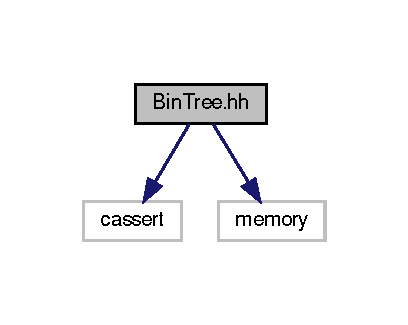
\includegraphics[width=196pt]{_bin_tree_8hh__incl}
\end{center}
\end{figure}
\subsection*{Clases}
\begin{DoxyCompactItemize}
\item 
class \hyperlink{class_bin_tree}{Bin\+Tree$<$ T $>$}
\end{DoxyCompactItemize}

\hypertarget{_cjt___clusters_8hh}{}\section{Referencia del Archivo Cjt\+\_\+\+Clusters.\+hh}
\label{_cjt___clusters_8hh}\index{Cjt\+\_\+\+Clusters.\+hh@{Cjt\+\_\+\+Clusters.\+hh}}


Especificación de la clase \hyperlink{class_cjt___clusters}{Cjt\+\_\+\+Clusters}.  


Dependencia gráfica adjunta para Cjt\+\_\+\+Clusters.\+hh\+:\nopagebreak
\begin{figure}[H]
\begin{center}
\leavevmode
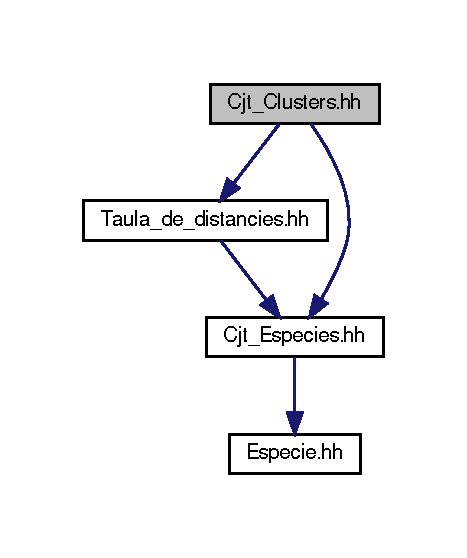
\includegraphics[width=224pt]{_cjt___clusters_8hh__incl}
\end{center}
\end{figure}
\subsection*{Clases}
\begin{DoxyCompactItemize}
\item 
class \hyperlink{class_cjt___clusters}{Cjt\+\_\+\+Clusters}
\begin{DoxyCompactList}\small\item\em Representa una \hyperlink{class_cjt___clusters}{Cjt\+\_\+\+Clusters}. \end{DoxyCompactList}\end{DoxyCompactItemize}
\subsection*{defines}
\begin{DoxyCompactItemize}
\item 
\#define \hyperlink{_cjt___clusters_8hh_ab12f5a8f10a954fe712afecc6ff2eca6}{C\+J\+T\+\_\+\+C\+L\+U\+S\+T\+E\+R\+S\+\_\+\+HH}
\end{DoxyCompactItemize}


\subsection{Descripción detallada}
Especificación de la clase \hyperlink{class_cjt___clusters}{Cjt\+\_\+\+Clusters}. 



\subsection{Documentación de los \textquotesingle{}defines\textquotesingle{}}
\mbox{\Hypertarget{_cjt___clusters_8hh_ab12f5a8f10a954fe712afecc6ff2eca6}\label{_cjt___clusters_8hh_ab12f5a8f10a954fe712afecc6ff2eca6}} 
\index{Cjt\+\_\+\+Clusters.\+hh@{Cjt\+\_\+\+Clusters.\+hh}!C\+J\+T\+\_\+\+C\+L\+U\+S\+T\+E\+R\+S\+\_\+\+HH@{C\+J\+T\+\_\+\+C\+L\+U\+S\+T\+E\+R\+S\+\_\+\+HH}}
\index{C\+J\+T\+\_\+\+C\+L\+U\+S\+T\+E\+R\+S\+\_\+\+HH@{C\+J\+T\+\_\+\+C\+L\+U\+S\+T\+E\+R\+S\+\_\+\+HH}!Cjt\+\_\+\+Clusters.\+hh@{Cjt\+\_\+\+Clusters.\+hh}}
\subsubsection{\texorpdfstring{C\+J\+T\+\_\+\+C\+L\+U\+S\+T\+E\+R\+S\+\_\+\+HH}{CJT\_CLUSTERS\_HH}}
{\footnotesize\ttfamily \#define C\+J\+T\+\_\+\+C\+L\+U\+S\+T\+E\+R\+S\+\_\+\+HH}



Definición en la línea 8 del archivo Cjt\+\_\+\+Clusters.\+hh.


\hypertarget{_cjt___especies_8hh}{}\section{Referencia del Archivo Cjt\+\_\+\+Especies.\+hh}
\label{_cjt___especies_8hh}\index{Cjt\+\_\+\+Especies.\+hh@{Cjt\+\_\+\+Especies.\+hh}}


Especificación de la clase \hyperlink{class_cjt___especies}{Cjt\+\_\+\+Especies}.  


Dependencia gráfica adjunta para Cjt\+\_\+\+Especies.\+hh\+:\nopagebreak
\begin{figure}[H]
\begin{center}
\leavevmode
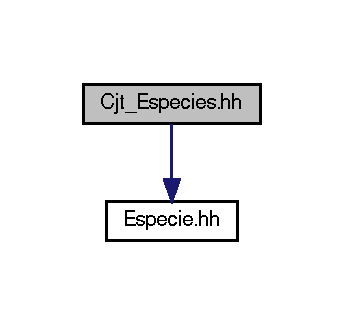
\includegraphics[width=165pt]{_cjt___especies_8hh__incl}
\end{center}
\end{figure}
\subsection*{Clases}
\begin{DoxyCompactItemize}
\item 
class \hyperlink{class_cjt___especies}{Cjt\+\_\+\+Especies}
\begin{DoxyCompactList}\small\item\em Representa una \hyperlink{class_cjt___especies}{Cjt\+\_\+\+Especies}. \end{DoxyCompactList}\end{DoxyCompactItemize}


\subsection{Descripción detallada}
Especificación de la clase \hyperlink{class_cjt___especies}{Cjt\+\_\+\+Especies}. 


\hypertarget{_especie_8hh}{}\section{Referencia del Archivo Especie.\+hh}
\label{_especie_8hh}\index{Especie.\+hh@{Especie.\+hh}}


Especificación de la clase \hyperlink{class_especie}{Especie}.  


\subsection*{Clases}
\begin{DoxyCompactItemize}
\item 
class \hyperlink{class_especie}{Especie}
\begin{DoxyCompactList}\small\item\em Representa una especie. \end{DoxyCompactList}\end{DoxyCompactItemize}


\subsection{Descripción detallada}
Especificación de la clase \hyperlink{class_especie}{Especie}. 


\hypertarget{program_8cc}{}\section{Referencia del Archivo program.\+cc}
\label{program_8cc}\index{program.\+cc@{program.\+cc}}


Programa principal para el ejercicio {\itshape Practica P\+R\+O2.\+Primavera 2020}.  


Dependencia gráfica adjunta para program.\+cc\+:
\nopagebreak
\begin{figure}[H]
\begin{center}
\leavevmode
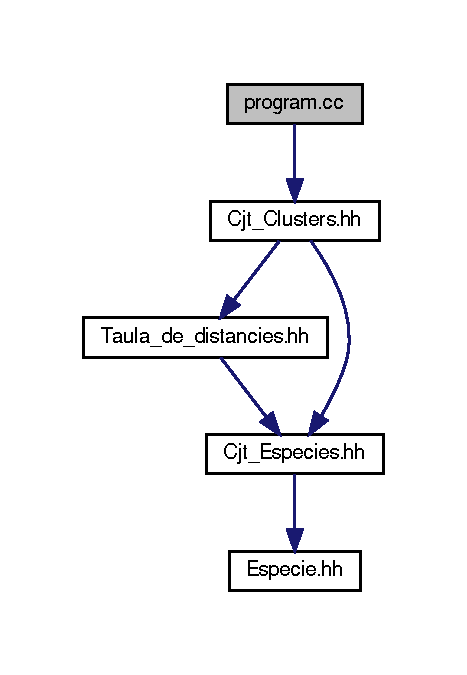
\includegraphics[width=224pt]{program_8cc__incl}
\end{center}
\end{figure}
\subsection*{Funciones}
\begin{DoxyCompactItemize}
\item 
void \hyperlink{program_8cc_a1a078453d3bb294251b421f3b4cf7f3c}{crea\+\_\+especie} (int k, \hyperlink{class_cjt___especies}{Cjt\+\_\+\+Especies} \&Mostra, \hyperlink{class_taula__de__distancies}{Taula\+\_\+de\+\_\+distancies} \&Taula, string ID, string gen)
\item 
int \hyperlink{program_8cc_ae66f6b31b5ad750f1fe042a706a4e3d4}{main} ()
\end{DoxyCompactItemize}


\subsection{Descripción detallada}
Programa principal para el ejercicio {\itshape Practica P\+R\+O2.\+Primavera 2020}. 



\subsection{Documentación de las funciones}
\mbox{\Hypertarget{program_8cc_a1a078453d3bb294251b421f3b4cf7f3c}\label{program_8cc_a1a078453d3bb294251b421f3b4cf7f3c}} 
\index{program.\+cc@{program.\+cc}!crea\+\_\+especie@{crea\+\_\+especie}}
\index{crea\+\_\+especie@{crea\+\_\+especie}!program.\+cc@{program.\+cc}}
\subsubsection{\texorpdfstring{crea\+\_\+especie()}{crea\_especie()}}
{\footnotesize\ttfamily void crea\+\_\+especie (\begin{DoxyParamCaption}\item[{int}]{k,  }\item[{\hyperlink{class_cjt___especies}{Cjt\+\_\+\+Especies} \&}]{Mostra,  }\item[{\hyperlink{class_taula__de__distancies}{Taula\+\_\+de\+\_\+distancies} \&}]{Taula,  }\item[{string}]{ID,  }\item[{string}]{gen }\end{DoxyParamCaption})}



Definición en la línea 18 del archivo program.\+cc.


\begin{DoxyCode}
18                                                                                                   \{
19     \textcolor{keywordtype}{bool} creado = Mostra.\hyperlink{class_cjt___especies_a39a4191697228fea8780516f4cd5da85}{existe\_especie}(ID);
20     \textcolor{keywordflow}{if} (creado) \{
21         cout << \textcolor{stringliteral}{"ERROR: La especie "} << ID << \textcolor{stringliteral}{" ya existe."} << endl;
22     \}
23     \textcolor{keywordflow}{else} \{
24         Mostra.\hyperlink{class_cjt___especies_a8c90cec35ff5469f0b8e193308569e4b}{crea\_especie}(ID, gen, k);
25         Taula.\hyperlink{class_taula__de__distancies_a6202c78b8a7c330d1be356d86e644a89}{afegeix\_especie}(ID, Mostra);
26     \}
27 \}
\end{DoxyCode}
\mbox{\Hypertarget{program_8cc_ae66f6b31b5ad750f1fe042a706a4e3d4}\label{program_8cc_ae66f6b31b5ad750f1fe042a706a4e3d4}} 
\index{program.\+cc@{program.\+cc}!main@{main}}
\index{main@{main}!program.\+cc@{program.\+cc}}
\subsubsection{\texorpdfstring{main()}{main()}}
{\footnotesize\ttfamily int main (\begin{DoxyParamCaption}{ }\end{DoxyParamCaption})}



Definición en la línea 29 del archivo program.\+cc.


\begin{DoxyCode}
29             \{
30     \textcolor{keywordtype}{int} k;
31     cin >> k;
32     \hyperlink{class_cjt___especies}{Cjt\_Especies} Mostra;
33     \hyperlink{class_cjt___clusters}{Cjt\_Clusters} Arbre;
34     \hyperlink{class_taula__de__distancies}{Taula\_de\_distancies} Taula;
35     \textcolor{keywordtype}{string} ordre;
36     cin >> ordre;
37     \textcolor{keywordflow}{while} (ordre != \textcolor{stringliteral}{"fin"}) \{
38         \textcolor{keywordflow}{if} (ordre == \textcolor{stringliteral}{"crea\_especie"}) \{
39             \textcolor{keywordtype}{string} ID, gen;
40             cin >> ID >> gen;
41             cout << \textcolor{stringliteral}{"# "} << ordre <<\textcolor{stringliteral}{" "} << ID << \textcolor{stringliteral}{" "} << gen << endl;
42             \hyperlink{program_8cc_a1a078453d3bb294251b421f3b4cf7f3c}{crea\_especie}(k, Mostra, Taula, ID, gen);
43         \}
44         \textcolor{keywordflow}{else} \textcolor{keywordflow}{if} (ordre == \textcolor{stringliteral}{"obtener\_gen"}) \{
45             \textcolor{keywordtype}{string} ID;
46             cin >> ID;
47             cout << \textcolor{stringliteral}{"# "} << ordre << \textcolor{stringliteral}{" "} << ID << endl;
48             \textcolor{keywordtype}{bool} existe = Mostra.\hyperlink{class_cjt___especies_a39a4191697228fea8780516f4cd5da85}{existe\_especie}(ID);
49             \textcolor{keywordflow}{if} (existe) \{
50                 \textcolor{keywordtype}{string} gen;
51                 gen = Mostra.\hyperlink{class_cjt___especies_af5821877f200218836053864ba8e9462}{obtener\_gen}(ID);
52                 cout << gen << endl;
53             \}
54             \textcolor{keywordflow}{else} cout << \textcolor{stringliteral}{"ERROR: La especie "} << ID << \textcolor{stringliteral}{" no existe."} << endl;
55         \}
56         \textcolor{keywordflow}{else} \textcolor{keywordflow}{if} (ordre == \textcolor{stringliteral}{"distancia"}) \{
57             \textcolor{keywordtype}{string} ID1, ID2;
58             cin >> ID1 >> ID2;
59             cout << \textcolor{stringliteral}{"# "} << ordre << \textcolor{stringliteral}{" "} << ID1 << \textcolor{stringliteral}{" "} << ID2 << endl;
60             \textcolor{keywordtype}{bool} e1\_existe = Mostra.\hyperlink{class_cjt___especies_a39a4191697228fea8780516f4cd5da85}{existe\_especie}(ID1);
61             \textcolor{keywordtype}{bool} e2\_existe = Mostra.\hyperlink{class_cjt___especies_a39a4191697228fea8780516f4cd5da85}{existe\_especie}(ID2);
62             \textcolor{keywordflow}{if} (e1\_existe and e2\_existe) \{
63                 \textcolor{keywordtype}{double} dist;
64                 dist = Taula.\hyperlink{class_taula__de__distancies_af3dfa32f4b29765b4ad1968bbb17ee16}{distancia}(ID1,ID2); 
65                 cout << dist << endl;
66             \}
67             \textcolor{keywordflow}{else} \textcolor{keywordflow}{if} (not e1\_existe and e2\_existe) \{
68                 cout << \textcolor{stringliteral}{"ERROR: La especie "} << ID1 << \textcolor{stringliteral}{" no existe."} << endl;
69             \}
70             \textcolor{keywordflow}{else} \textcolor{keywordflow}{if} (e1\_existe and not e2\_existe) cout << \textcolor{stringliteral}{"ERROR: La especie "} << ID2 << \textcolor{stringliteral}{" no existe."} << 
      endl;
71             \textcolor{keywordflow}{else} cout << \textcolor{stringliteral}{"ERROR: La especie "} << ID1 << \textcolor{stringliteral}{" y la especie "} << ID2 << \textcolor{stringliteral}{" no existen."} << endl;
72         \}
73         
74         \textcolor{keywordflow}{else} \textcolor{keywordflow}{if} (ordre == \textcolor{stringliteral}{"elimina\_especie"}) \{
75             \textcolor{keywordtype}{string} ID;
76             cin >> ID;
77             cout << \textcolor{stringliteral}{"# "} << ordre << \textcolor{stringliteral}{" "} << ID << endl;
78             \textcolor{keywordtype}{bool} eliminado = Mostra.\hyperlink{class_cjt___especies_a39a4191697228fea8780516f4cd5da85}{existe\_especie}(ID);
79             \textcolor{keywordflow}{if} (eliminado) \{
80                 Taula.\hyperlink{class_taula__de__distancies_ab7b1113061a5022c4444ff299e143f50}{eliminar\_especie}(ID);
81                 Mostra.\hyperlink{class_cjt___especies_aef76f607ead23a635d7a8b2c9a844327}{elimina\_especie}(ID);
82             \}
83             \textcolor{keywordflow}{else} cout << \textcolor{stringliteral}{"ERROR: La especie "} << ID << \textcolor{stringliteral}{" no existe."} << endl;
84         \}
85         \textcolor{keywordflow}{else} \textcolor{keywordflow}{if} (ordre == \textcolor{stringliteral}{"existe\_especie"}) \{
86             \textcolor{keywordtype}{string} ID;
87             cin >> ID;
88             cout << \textcolor{stringliteral}{"# "} << ordre << \textcolor{charliteral}{' '} << ID << endl;
89             \textcolor{keywordtype}{bool} exist = Mostra.\hyperlink{class_cjt___especies_a39a4191697228fea8780516f4cd5da85}{existe\_especie}(ID);
90             \textcolor{keywordflow}{if} (exist) \{
91                 cout << \textcolor{stringliteral}{"SI"} << endl;
92             \}
93             \textcolor{keywordflow}{else} cout << \textcolor{stringliteral}{"NO"} << endl;
94         \}
95         \textcolor{keywordflow}{else} \textcolor{keywordflow}{if} (ordre == \textcolor{stringliteral}{"lee\_cjt\_especies"}) \{
96             \textcolor{keywordtype}{int} n;
97             cin >> n;
98             cout << \textcolor{stringliteral}{"# "} << ordre << endl;
99             Mostra.\hyperlink{class_cjt___especies_a341dfedcac85d19e084d68f7611af8f9}{eliminar\_totes}();
100             Taula.\hyperlink{class_taula__de__distancies_afb9dd4b7cca03fd7da25d60a8603e765}{buidar\_taula}();
101             \textcolor{keywordflow}{for} (\textcolor{keywordtype}{int} i = 0; i < n; ++i) \{
102                 \textcolor{keywordtype}{string} ID, gen;
103                 cin >> ID >> gen;
104                 \hyperlink{program_8cc_a1a078453d3bb294251b421f3b4cf7f3c}{crea\_especie}(k, Mostra, Taula, ID, gen);
105             \}
106         \}
107         \textcolor{keywordflow}{else} \textcolor{keywordflow}{if} (ordre == \textcolor{stringliteral}{"imprime\_cjt\_especies"}) \{
108             cout << \textcolor{stringliteral}{"# "} << ordre << endl;
109             Mostra.\hyperlink{class_cjt___especies_a61b0168970e926d3a27faf3f31ad2869}{imprime\_cjt\_especies}();
110         \}
111         \textcolor{keywordflow}{else} \textcolor{keywordflow}{if} (ordre == \textcolor{stringliteral}{"tabla\_distancias"}) \{
112             cout << \textcolor{stringliteral}{"# "} << ordre << endl;
113             \hyperlink{class_taula__de__distancies}{Taula\_de\_distancies} taula\_aux = Taula;
114             taula\_aux.\hyperlink{class_taula__de__distancies_a494108f6c1af52fd9f8032d1ec78fc32}{tabla\_distancias}();
115         \}
116         \textcolor{keywordflow}{else} \textcolor{keywordflow}{if} (ordre == \textcolor{stringliteral}{"inicializa\_clusters"}) \{
117             cout << \textcolor{stringliteral}{"# "} << ordre << endl;
118             \hyperlink{class_taula__de__distancies}{Taula\_de\_distancies} taula\_aux = Taula;
119             Arbre.\hyperlink{class_cjt___clusters_a7dec4a423a1dbcf6d0351e00dd653eee}{inicializa\_clusters}(Mostra, Taula);
120             taula\_aux.\hyperlink{class_taula__de__distancies_a494108f6c1af52fd9f8032d1ec78fc32}{tabla\_distancias}();
121         \}
122         \textcolor{keywordflow}{else} \textcolor{keywordflow}{if} (ordre == \textcolor{stringliteral}{"ejecuta\_paso\_wpgma"}) \{
123             cout << \textcolor{stringliteral}{"# "} << ordre << endl;
124             \textcolor{keywordtype}{int} num\_c = Arbre.\hyperlink{class_cjt___clusters_ad00d2fe80f0b0dc1e593a91f8be6b761}{numero\_clusters}();
125             \textcolor{keywordflow}{if} (num\_c > 2) \{
126                 Arbre.\hyperlink{class_cjt___clusters_a1656b81e5200625b44c8f138c09af068}{ejecutar\_paso\_wpgma}();
127                 Arbre.\hyperlink{class_cjt___clusters_a6a261f0f5ca471e257d6b17e91b4887a}{taula\_clusters\_imprime}();
128             \}
129             \textcolor{keywordflow}{else} cout << \textcolor{stringliteral}{"ERROR: num\_clusters <= 1"} << endl;
130         \}
131         \textcolor{keywordflow}{else} \textcolor{keywordflow}{if} (ordre == \textcolor{stringliteral}{"imprime\_cluster"}) \{
132             \textcolor{keywordtype}{string} id;
133             cin >> id;
134             cout << \textcolor{stringliteral}{"# "} << ordre << \textcolor{stringliteral}{" "} << \textcolor{keywordtype}{id} << endl;
135             \textcolor{keywordflow}{if} (Arbre.\hyperlink{class_cjt___clusters_a4fcda36a68e8fe48d787dfd14e9b222b}{existe\_cluster}(\textcolor{keywordtype}{id})) \{
136                 \hyperlink{class_bin_tree}{BinTree<pair<string,double>}> aux = Arbre.
      \hyperlink{class_cjt___clusters_aca3506a7084d53e251ff052b0bbaf5bb}{retorna\_subarb}(\textcolor{keywordtype}{id});
137                 Arbre.\hyperlink{class_cjt___clusters_a19510eceda5d5bf39d7091a28bf5f00c}{imprime\_cluster\_aux}(aux);
138             \}
139             \textcolor{keywordflow}{else} cout << \textcolor{stringliteral}{"ERROR: El cluster "} << \textcolor{keywordtype}{id} << \textcolor{stringliteral}{" no existe."} << endl;
140         \}
141         \textcolor{keywordflow}{else} \textcolor{keywordflow}{if} (ordre == \textcolor{stringliteral}{"imprime\_arbol\_filogenetico"}) \{
142             cout << \textcolor{stringliteral}{"# "} << ordre << endl;
143             Arbre.\hyperlink{class_cjt___clusters_a7dec4a423a1dbcf6d0351e00dd653eee}{inicializa\_clusters}(Mostra, Taula);
144             \textcolor{keywordtype}{int} num\_c = Arbre.\hyperlink{class_cjt___clusters_ad00d2fe80f0b0dc1e593a91f8be6b761}{numero\_clusters}();
145             \textcolor{keywordflow}{if} (num\_c > 0) \{
146                 \textcolor{keywordflow}{while} (num\_c > 1) \{
147                     Arbre.\hyperlink{class_cjt___clusters_a1656b81e5200625b44c8f138c09af068}{ejecutar\_paso\_wpgma}();
148                     num\_c = Arbre.\hyperlink{class_cjt___clusters_ad00d2fe80f0b0dc1e593a91f8be6b761}{numero\_clusters}();
149                 \}
150                 Arbre.\hyperlink{class_cjt___clusters_a95262506a2fdc5455ce104fb84649ee9}{imprime\_arbol\_filogenetico}();
151             \}
152             \textcolor{keywordflow}{else} cout << \textcolor{stringliteral}{"ERROR: El conjunto de clusters es vacio."} << endl;
153         \}
154         cin >> ordre;
155         cout << endl;
156     \}
157 \}
\end{DoxyCode}

\hypertarget{_taula__de__distancies_8hh}{}\section{Referencia del Archivo Taula\+\_\+de\+\_\+distancies.\+hh}
\label{_taula__de__distancies_8hh}\index{Taula\+\_\+de\+\_\+distancies.\+hh@{Taula\+\_\+de\+\_\+distancies.\+hh}}


Especificación de la clase \hyperlink{class_taula__de__distancies}{Taula\+\_\+de\+\_\+distancies}.  


Dependencia gráfica adjunta para Taula\+\_\+de\+\_\+distancies.\+hh\+:\nopagebreak
\begin{figure}[H]
\begin{center}
\leavevmode
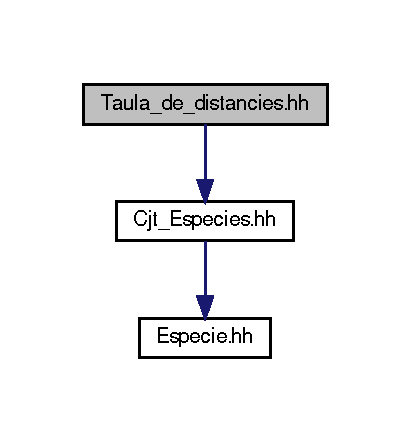
\includegraphics[width=197pt]{_taula__de__distancies_8hh__incl}
\end{center}
\end{figure}
\subsection*{Clases}
\begin{DoxyCompactItemize}
\item 
class \hyperlink{class_taula__de__distancies}{Taula\+\_\+de\+\_\+distancies}
\begin{DoxyCompactList}\small\item\em Representa una \hyperlink{class_taula__de__distancies}{Taula\+\_\+de\+\_\+distancies}. \end{DoxyCompactList}\end{DoxyCompactItemize}


\subsection{Descripción detallada}
Especificación de la clase \hyperlink{class_taula__de__distancies}{Taula\+\_\+de\+\_\+distancies}. 


%--- End generated contents ---

% Index
\backmatter
\newpage
\phantomsection
\clearemptydoublepage
\addcontentsline{toc}{chapter}{Índice}
\printindex

\end{document}
